%%%%%%%%%%%%%%%%%%%%%%%%%%%%%%%%%%%%%%%%%
% Memo
% LaTeX Template
% Version 1.0 (30/12/13)
%
% This template has been downloaded from:
% http://www.LaTeXTemplates.com
%
% Original author:
% Rob Oakes (http://www.oak-tree.us) with modifications by:
% Vel (vel@latextemplates.com)
%
% License:
% CC BY-NC-SA 3.0 (http://creativecommons.org/licenses/by-nc-sa/3.0/)
%
%%%%%%%%%%%%%%%%%%%%%%%%%%%%%%%%%%%%%%%%%

\documentclass[letterpaper,11pt]{texMemo} % Set the paper size (letterpaper, a4paper, etc) and font size (10pt, 11pt or 12pt)

\usepackage{fancyhdr}
\usepackage{fancybox}
\usepackage{longtable}
\usepackage{amsmath}
%----------------------------------------------------------------------------------------
%	MEMO INFORMATION
%----------------------------------------------------------------------------------------

\memoto{Luis Andr\'es Valido Fajardo. luis.valido@umcc.cu (53694742)} % Recipient(s)

\memofrom{Josval Díaz Blanco} % Sender(s)

\memosubject{Guía de Aprendizaje para Concursantes ICPC y IOI: Búsqueda Binaria } % Memo subject

\memodate{\today} % Date, set to \today for automatically printing todays date

\logo{
\includegraphics[scale=0.5]{img/icpc}} % Institution logo at the top right of the memo, comment out this line for no logo

%----------------------------------------------------------------------------------------

\begin{document}

%\AddToShipoutPicture{\BackgroundPic}
\maketitle % Print the memo header information
%\tableofcontents

\pagebreak

\pagestyle{fancy}
\fancyhead[LO,CE]{ 
\includegraphics[scale=0.03]{img/logo1}}
\fancyhead[RO,CE]{
\includegraphics[scale=0.1]{img/icpc}}
\fancyfoot[LO,CE]{\textbf{Autor:} Luis Andrés Valido Fajardo \\ \textbf{Email:} luis.valido1989@gmail.com \\ \textbf{Teléfono:} 53694742}
\fancyfoot[RO,CE]{\emph{Existen 10 tipos de personas Las que \\saben binario y LAS QUE NO}}
\fancypagestyle{plain}{\pagestyle{fancy}}



%\lhead{ }
%\rhead{  }

%\fancyfoot[L]{}
%\fancyfoot[R]{\textbf{Autor:} Luis Andrés Valido Fajardo \\ \textbf{Email:} luis.valido@umcc.cu}
%----------------------------------------------------------------------------------------
%	MEMO CONTENT
%----------------------------------------------------------------------------------------


\section{Introducción}
En geometría computacional, un algoritmo de línea de barrido (\emph{sweep line}) o un algoritmo de barrido plano es un paradigma algorítmico que utiliza una línea de barrido conceptual o una superficie de barrido para resolver varios problemas en el espacio euclidiano. Es una de las técnicas críticas en geometría computacional.
\section{Conocimientos previos}
\subsection{Distancia euclidiana}
La distancia euclidiana es simplemente la distancia entre dos puntos cuando se calcula haciendo uso del teorema de Pitágoras. Viene dado por la raíz cuadrada de $(x_1 - x_2)^2 + (y_1 - y_2)^2$.

% TODO: \usepackage{graphicx} required
\begin{figure}[h!]
	\centering
	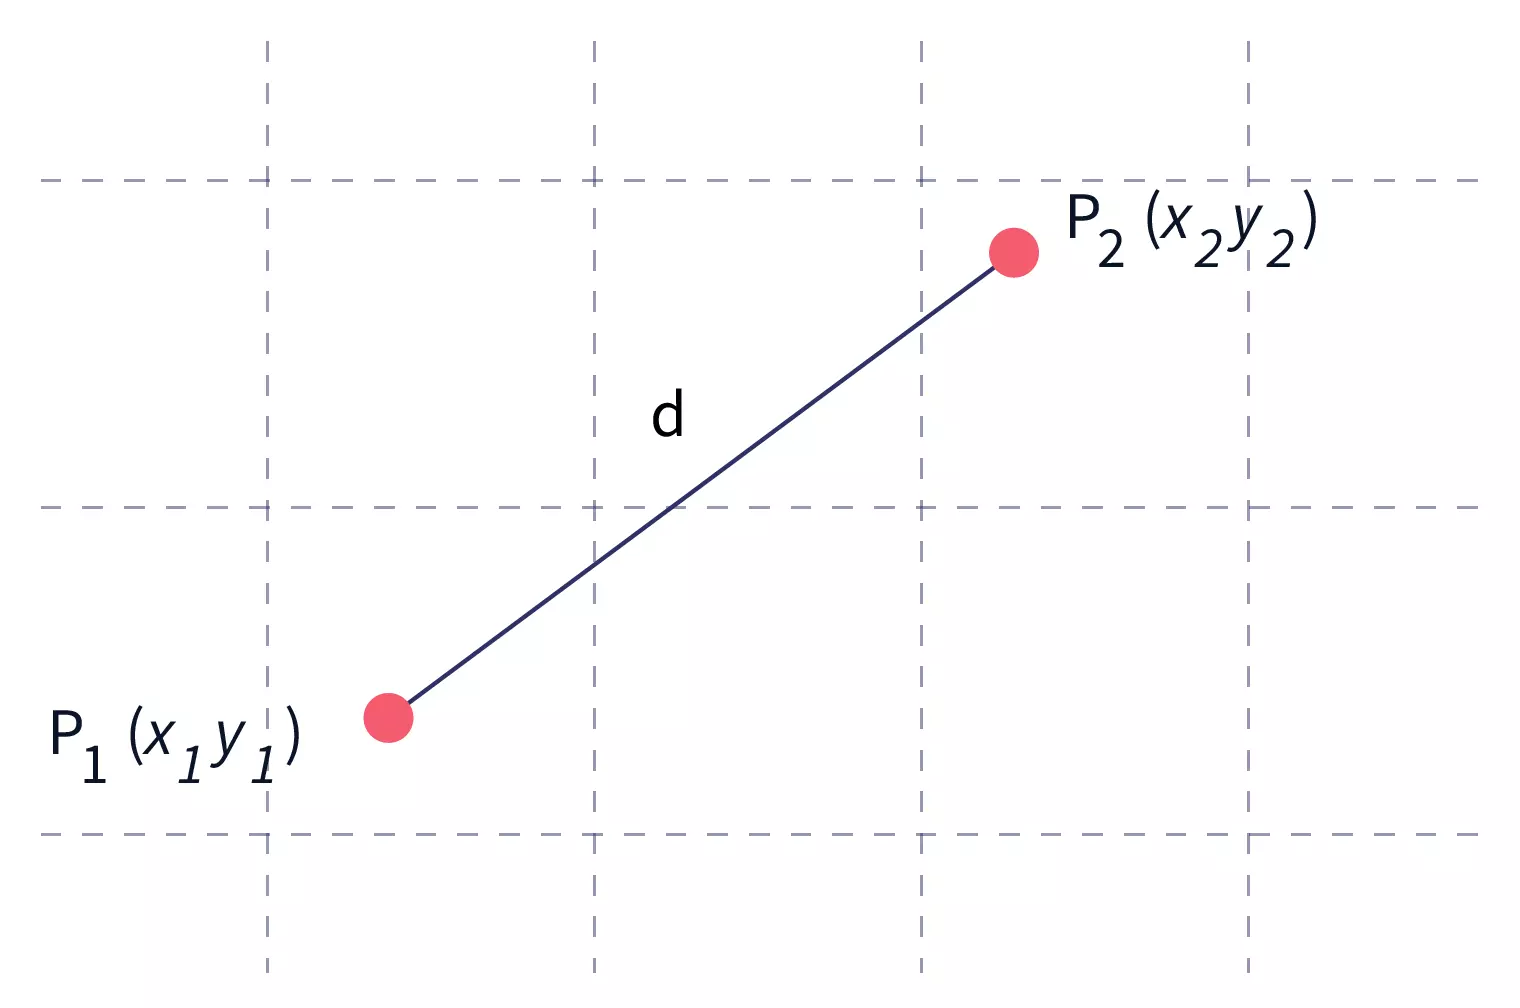
\includegraphics[width=0.35\linewidth]{img/distancia_euclidiana}
	\label{fig:distanciaeuclidiana}
\end{figure}


\subsection{Distancia Manhattan}
La distancia de Manhattan es la distancia recorrida cuando te mueves solo verticalmente o solo horizontalmente. Está dado por $ |x_1-x_2| + |y_1-y_2|$.

% TODO: \usepackage{graphicx} required
\begin{figure}[h!]
	\centering
	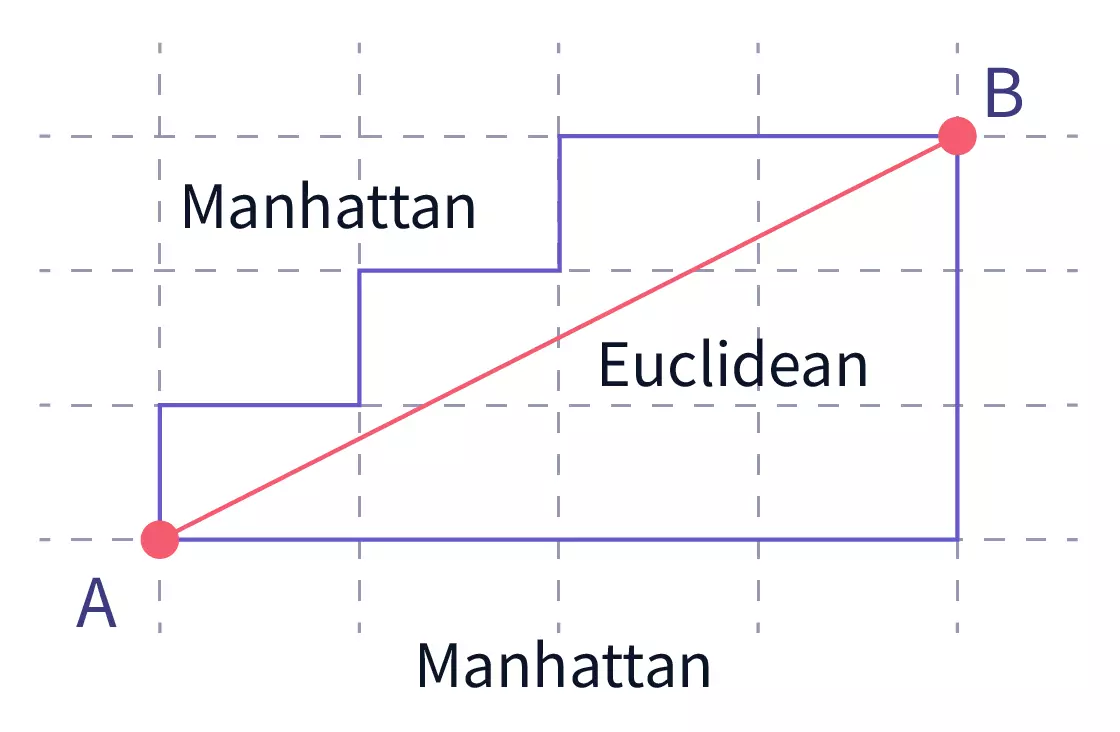
\includegraphics[width=0.35\linewidth]{img/distancia_manhattan}
	\label{fig:distanciamanhattan}
\end{figure}

\subsection{Árbol de expansión mínima}

Dado un grafo conexo y no dirigido, un árbol recubridor, árbol de cobertura o árbol de expansión de ese grafo es un subgrafo que tiene que ser un árbol y contener todos los vértices del grafo
inicial. Cada arista tiene asignado un peso proporcional entre ellos, que es un número representativo de algún objeto, distancia, etc.; y se usa para asignar un peso total al árbol recubridor mínimo
computando la suma de todos los pesos de las aristas del árbol en cuestión. Un árbol recubridor
mínimo o un árbol de expansión mínimo es un árbol recubridor que pesa menos o igual que todos
los otros árboles recubridores. Todo grafo tiene un bosque recubridor mínimo.

\section{Desarrollo}
Este enfoque puede rastrearse hasta los algoritmos de línea de exploración de representación en gráficos por computadora, seguido de la explotación de este enfoque en los primeros algoritmos de diseño de diseño de circuitos integrados, en los que se procesaba una descripción geométrica de un circuito integrado en tiras paralelas porque la descripción completa no cabía en la memoria. .

La idea detrás de los algoritmos de este tipo es imaginar que una línea (a menudo una línea vertical) es barrida o movida a través del plano, deteniéndose en algunos puntos. Las operaciones geométricas están restringidas a los objetos geométricos que intersecan o se encuentran en las inmediaciones de la línea de barrido cada vez que se detiene, y la solución completa está disponible una vez que la línea ha pasado por todos los objetos.

En términos prácticos no la podemos mover de forma continua ya que hay infinitos puntos, por lo que solo la vamos a mover de forma discreta en los lugares de interés, a los que llamaremos \textbf{eventos}.

Lo mínimo que esos eventos necesitan guardar es el tiempo en el que ocurren, y la forma usual de procesarlos es ordenarlos por dicho tiempo de menor a mayor, iterar por todos ellos y mantener cierta información global relativa al problema que irá cambiando entre evento y \textbf{evento}.

La idea de tales algoritmos es representar una instancia del problema como un conjunto de \textbf{eventos} que corresponden a puntos en el plano. Los \textbf{eventos} se procesan en orden creciente según sus coordenadas $x$ o $y$.

Como ejemplo, considere el siguiente problema: \emph{Hay una empresa que tiene $N$ empleados, y sabemos para cada empleado su hora de entrada y salida en un día determinado. Nuestra tarea es calcular el número máximo de empleados que estaban en la oficina al mismo tiempo.}

El problema se puede resolver modelando la situación de modo que a cada empleado se le asignen dos eventos que correspondan a sus tiempos de llegada y salida. Después de ordenar los eventos, los revisamos y hacemos un seguimiento de la cantidad de personas en la oficina. Por ejemplo como se muestra en la siguiente tabla:



\begin{longtable}{ccc}
	
	\textbf{Empleado}& \textbf{Tiempo de llegada}  & \textbf{Tiempo de salida}  \\
	
	John & 10 & 15  \\

	Maria & 6 & 12 \\

	Peter & 14  & 16 \\
	
	Lisa & 5  &  13 \\
	
\end{longtable}

corresponde a los siguientes eventos:

% TODO: \usepackage{graphicx} required
\begin{figure}[h!]
	\centering
	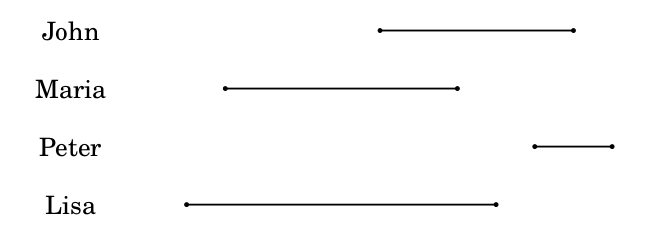
\includegraphics[width=0.5\linewidth]{img/example_sweep_line}
	\label{fig:examplesweepline}
\end{figure}

Revisamos los eventos de izquierda a derecha y mantenemos un contador. Siempre cuando llega una persona, aumentamos el valor del contador en uno, y cuando una persona se va, disminuimos el valor del contador en uno. La respuesta al problema es el valor máximo del contador durante el algoritmo.

En el ejemplo, los eventos se procesan de la siguiente manera:

\begin{figure}[h!]
	\centering
	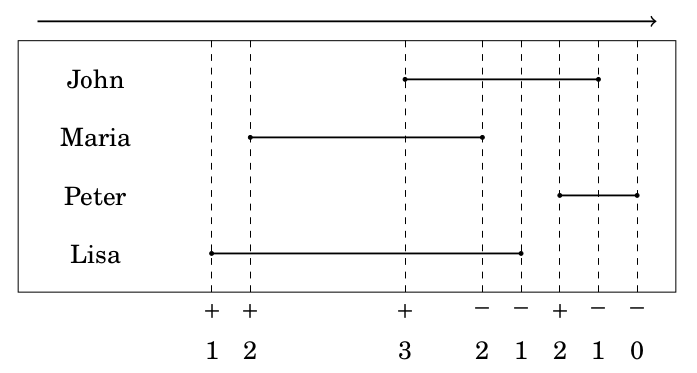
\includegraphics[width=0.5\linewidth]{img/example_sweep_line2}
	\label{fig:examplesweepline2}
\end{figure}

Los símbolos $+$ y $-$ indican si el valor del contador aumenta o disminuye, y el valor del contador se muestra a continuación. El valor máximo del contador es 3 entre la llegada de Juan y la salida de María.

El tiempo de ejecución del algoritmo es O ($n\log n$), porque ordenar los eventos toma O($n\log n$) tiempo y el resto del algoritmo toma O($n$) tiempo. Donde $n$ es el doble de personas ya que por cada persona se registra dos \textbf{eventos}.

El algoritmo de barrido de línea se utiliza para resolver problemas como el par más cercano, las intersecciones de segmentos de línea, la unión de rectángulos, la envoltura convexa, el árbol de expansión mínimo de Manhattan los cuales vamos analizar su solución aplicando este paradigma algorítmico.

\subsection{Par más cercano (\emph{Closest pair})}
Dado un conjunto de puntos, encuentre el par más cercano (con cualquier métrica). Por supuesto, esto puede resolverse en tiempo O($N^2$) considerando todos los pares, pero un barrido de línea puede reducirlo a O($N\log N$).

Supongamos que hemos procesado los puntos $1$ a $N-1$ (ordenados por $x$) y la distancia más corta que hemos encontrado hasta ahora es $h$. Ahora procesamos el punto $N$ e intentamos encontrar un punto más cercano a él que $h$. Mantenemos un conjunto de todos los puntos ya procesados cuyas coordenadas $X$ están dentro de $h$ del punto $N$, como se muestra en el rectángulo gris claro. A medida que se procesa cada punto, se agrega al conjunto, y cuando pasamos al siguiente punto o cuando se disminuye $h$, los puntos se eliminan del conjunto. El conjunto está ordenado por la coordenada $y$. Un árbol binario balanceado es adecuado para esto y representa el factor $\log N$.

% TODO: \usepackage{graphicx} required
\begin{figure}[h!]
	\centering
	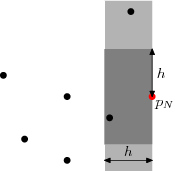
\includegraphics[width=0.2\linewidth]{img/closest}
	\label{fig:closest}
\end{figure}

Para buscar puntos más cercanos que $h$ al punto $N$, solo necesitamos considerar puntos en el conjunto activo y, además, solo necesitamos considerar puntos cuyas coordenadas y estén en el rango $N_y - h$ a $N_y + h$ (aquellos en el rectángulo gris oscuro) . Este rango se puede extraer del conjunto ordenado en tiempo O($\log N$), pero lo que es más importante, el número de elementos es O($1$) (el máximo exacto dependerá de la métrica utilizada), porque la separación entre dos puntos cualesquiera en el conjunto es al menos $h$. De ello se deduce que la búsqueda de cada punto requiere un tiempo O($\log N$), dando un total de O($N\log N$).

\subsection{Intersecciones de segmento de línea}
Comenzaremos considerando el problema de devolver todas las intersecciones en un conjunto de segmentos de línea horizontales y verticales. Dado que las líneas horizontales no tienen una sola coordenada X, tenemos que abandonar la idea de clasificar los objetos por X. En su lugar, tenemos la idea de un evento: una coordenada X en la que sucede algo interesante. En este caso, los tres tipos de eventos son: inicio de una línea horizontal, final de una línea horizontal y una línea vertical. A medida que se mueve la línea de barrido, mantendremos un conjunto activo de líneas horizontales cortadas por la línea de barrido, ordenadas por valor Y (las líneas rojas en la figura).

% TODO: \usepackage{graphicx} required
\begin{figure}[h!]
	\centering
	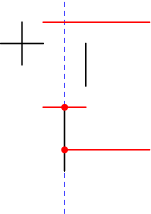
\includegraphics[width=0.2\linewidth]{img/linesvh}
	\label{fig:linesvh}
\end{figure}

Para manejar cualquiera de los eventos de línea horizontal, simplemente necesitamos agregar o eliminar un elemento del conjunto. Nuevamente, podemos usar un árbol binario balanceado para garantizar el tiempo O ($\log N$) para estas operaciones. Cuando llegamos a una línea vertical, una búsqueda de rango proporciona inmediatamente todas las líneas horizontales que corta. Si los segmentos horizontales o verticales pueden superponerse, se requiere algo de trabajo adicional, y también debemos considerar si se considera que las líneas con extremos coincidentes se cruzan, pero nada de esto afecta la complejidad computacional.

Si se requieren las intersecciones en sí, esto toma un tiempo O ($N \log N + I$) para las intersecciones $I$. Al aumentar la estructura del árbol binario (específicamente, al almacenar el tamaño de cada subárbol en la raíz de ese subárbol), es posible contar las intersecciones en tiempo O($N \log N$).

En el caso más general, las líneas no necesitan ser horizontales o verticales, por lo que las líneas en el conjunto activo pueden intercambiar lugares cuando se cruzan. En lugar de tener todos los eventos ordenados previamente, tenemos que usar una cola de prioridad y agregar y eliminar dinámicamente los eventos de intersección. En cualquier momento, la cola de prioridad contiene eventos para los puntos finales de los segmentos de línea, pero también para los puntos de intersección de los elementos adyacentes del conjunto activo (siempre que estén en el futuro). Dado que hay eventos O($N + I$) que se alcanzarán, y cada uno requiere un tiempo O($\log N$) para actualizar el conjunto activo y la cola de prioridad, este algoritmo toma un tiempo O($N \log N + I \log N$). La siguiente figura muestra los eventos futuros en la cola de prioridad (puntos azules); tenga en cuenta que no todas las intersecciones futuras están en la cola, ya sea porque una de las líneas aún no está activa o porque las dos líneas aún no son adyacentes en la lista activa.

% TODO: \usepackage{graphicx} required
\begin{figure}[h!]
	\centering
	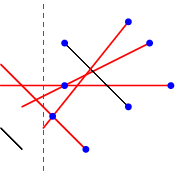
\includegraphics[width=0.2\linewidth]{img/lines}
	\label{fig:lines}
\end{figure}


\subsection{Área de la unión de rectángulos}
Dado un conjunto de rectángulos alineados con el eje, ¿cuál es el área de su unión? Al igual que el problema de la intersección de líneas, podemos manejar esto tratando con eventos y conjuntos activos. Cada rectángulo tiene dos eventos: borde izquierdo y borde derecho. Cuando cruzamos el borde izquierdo, el rectángulo se agrega al conjunto activo. Cuando cruzamos el borde derecho, se elimina del conjunto activo.

% TODO: \usepackage{graphicx} required
\begin{figure}[h!]
	\centering
	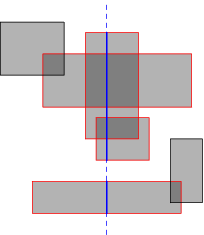
\includegraphics[width=0.2\linewidth]{img/rects}
	\label{fig:rects}
\end{figure}

Ahora sabemos qué rectángulos corta la línea de barrido (roja en el diagrama), pero en realidad queremos saber la longitud de la línea de barrido que se corta (la longitud total de los segmentos azules sólidos). Al multiplicar esta longitud por la distancia horizontal entre eventos, se obtiene el área barrida entre esos dos eventos.

Podemos determinar la longitud de corte ejecutando el mismo algoritmo en un bucle interno, pero girado 90 grados. Ignore los rectángulos inactivos y considere una línea de barrido horizontal que se mueve de arriba hacia abajo. Los eventos ahora son los bordes horizontales de los rectángulos activos, y cada vez que cruzamos uno, podemos simplemente incrementar o disminuir un contador que dice cuántos rectángulos se superponen en el punto actual. La longitud de corte aumenta siempre que el contador no sea cero. Por supuesto, no lo aumentamos continuamente, sino mientras pasamos de un evento a otro.

Con las estructuras de datos correctas, esto se puede implementar en tiempo O($N^2$) (sugerencia: use una matriz booleana para almacenar el conjunto activo en lugar de un árbol binario balanceado, y ordene previamente todo el conjunto de bordes horizontales). De hecho, el barrido de la línea interna se puede reemplazar con una manipulación inteligente del árbol binario para reducir el tiempo total a O ($N \log N$), pero eso es más un problema en las estructuras de datos que en la geometría, y se deja como un ejercicio para el lector. El algoritmo también se puede adaptar para responder preguntas similares, como la longitud total del perímetro de la unión o el número máximo de rectángulos que se superponen en cualquier punto.

\subsection{Envoltura convexa (\emph{Convex hull})}
La envoltura convexa de un conjunto de puntos es el polígono convexo más pequeño que rodea todo el conjunto y tiene una serie de aplicaciones prácticas. Un método eficiente que se usa a menudo en los desafíos es el escaneo de Graham, que requiere una clasificación por ángulo. Esto no es tan fácil como parece al principio, ya que calcular los ángulos reales es costoso e introduce problemas de error numérico. Un algoritmo más simple pero igualmente eficiente se debe a Andrew, y requiere solo una ordenación por $X$ para un barrido de línea aunque el artículo original de Andrew ordena por $Y$ y tiene algunas optimizaciones que no discutiré aquí.

El algoritmo de Andrew divide la envoltura convexa en dos partes, la envoltura superior y el inferior. Por lo general, estos se encuentran en los extremos, pero si más de un punto tiene una coordenada X mínima (o máxima), entonces se unen mediante un segmento de línea vertical. Describiremos cómo construir la envoltura superior; la envoltura inferior se puede construir de manera similar y, de hecho, se puede construir en el mismo bucle.

Para construir el casco superior, comenzamos con el punto con la coordenada $X$ mínima, rompiendo los lazos tomando la coordenada $Y$ más grande. Después de esto, los puntos se agregan en el orden de la coordenada $X$ (siempre tomando el valor Y más grande cuando varios puntos tienen el mismo valor $X$). Por supuesto, a veces esto hará que el casco se vuelva cóncavo en lugar de convexo:


% TODO: \usepackage{graphicx} required
\begin{figure}[h!]
	\centering
	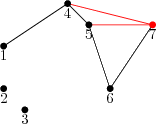
\includegraphics[width=0.2\linewidth]{img/uhull}
	\label{fig:uhull}
\end{figure}


El camino negro muestra el casco actual. Después de agregar el punto 7, verificamos si el último triángulo (5, 6, 7) es convexo. En este caso no lo es, por lo que eliminamos el penúltimo punto, es decir, el 6. El proceso se repite hasta encontrar un triángulo convexo. En este caso también examinamos (4, 5, 7) y eliminamos 5 antes de examinar (1, 4, 7) y encontrar que es convexo, antes de pasar al siguiente punto. Este es esencialmente el mismo procedimiento que se usa en la exploración de Graham, pero procediendo en el orden de la coordenada $X$ en lugar del orden del ángulo formado con el punto de partida. A primera vista, puede parecer que este proceso es O($N^2$) debido al bucle interno de retroceso, pero dado que ningún punto se puede eliminar más de una vez, en realidad es O($N$). El algoritmo general es O($N \log N$), porque los puntos deben ordenarse inicialmente por la coordenada $X$.

\subsection{Árbol de expansión mínimo de Manhattan}
Podemos crear algoritmos aún más potentes combinando un barrido de línea con un algoritmo de divide y vencerás. Un ejemplo es calcular el árbol de expansión mínimo de un conjunto de puntos, donde la distancia entre cualquier par de puntos es la distancia de Manhattan. Este es esencialmente el algoritmo presentado por Guibas y Stolfi.

Primero desglosamos esto en un problema más simple. Los algoritmos de árbol de expasión minima(\emph{MST}) estándar para grafos generales (p. ej., el algoritmo de Prim) pueden calcular el MST en tiempo O ($(E + N)\log N$) para aristas E. Si podemos explotar las propiedades geométricas para reducir el número de aristas a O($N$), entonces esto es simplemente O($N \log N$). De hecho, podemos considerar, para cada punto P, solo sus vecinos más cercanos en cada uno de los 8 octantes del plano (ver la figura a continuación). La figura muestra la situación en uno solo de los octantes, el Oeste-Noroeste. $Q$ es el vecino más cercano (con la línea discontinua que indica puntos a la misma distancia de Manhattan que $Q$), y $R$ es algún otro punto en el octante. Si $PR$ es una arista en un árbol de expansión, entonces puede eliminarse y reemplazarse por $PQ$ o $QR$ para producir un árbol de expansión mejor, porque la forma del octante garantiza que $|QR| = |PR|$. Por lo tanto, no necesitamos considerar $PR$ cuando construimos el árbol de expansión.

% TODO: \usepackage{graphicx} required
\begin{figure}[!h]
	\centering
	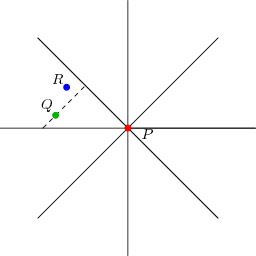
\includegraphics[width=0.25\linewidth]{img/octants}
	\label{fig:octants}
\end{figure}

Esto reduce el problema a encontrar el vecino más cercano en cada octante. Solo consideraremos el octante que se muestra; los otros no son diferentes y pueden manejarse por simetría. Debería quedar claro que dentro de este octante, encontrar el vecino más cercano es equivalente a simplemente encontrar el punto con el mayor valor de $x - y$, sujeto a un límite superior en $x + y$ y un límite inferior en $y$, y esta es la forma en el que consideraremos el problema.

Ahora imagine por el momento que el límite inferior de y no existe. En este caso podríamos resolver el problema para cada $P$ con bastante facilidad: barrer los puntos en orden creciente de $x + y$, y $Q$ será el punto con el mayor valor de $x - y$ de los vistos hasta ahora. Aquí es donde entra en juego el principio de divide y vencerás: dividimos el conjunto de puntos en dos mitades con una línea horizontal y resolvemos recursivamente el problema para cada mitad. Para los puntos $P$ en la mitad superior, no se necesita hacer nada más, porque los puntos en la mitad inferior no pueden jugar $Q$ con su $P$. Para la mitad inferior, debemos considerar que al ignorar la mitad superior hasta ahora, es posible que nos hayamos perdido algunos puntos más cercanos. Sin embargo, podemos tener en cuenta estos puntos de una manera similar a la anterior: recorrer todos los puntos en el orden $x + y$, siguiendo el mejor punto en la mitad superior (mayor valor $x - y$), y para cada punto en la mitad inferior, comprobando si este mejor punto de la mitad superior es mejor que el vecino actual.

Hasta ahora, he asumido alegremente que cualquier conjunto de puntos se puede dividir de manera eficiente en Y y también caminar en el orden $x + y$ sin decir cómo se debe hacer esto. De hecho, uno de los aspectos más hermosos de esta clase de algoritmos de divide y vencerás más barrido de línea es que tiene esencialmente la misma estructura que una ordenación por combinación, hasta el punto de que una ordenación por combinación $x + y$ puede ser doblado en el algoritmo de tal manera que cada subconjunto se ordena en $x + y$ justo cuando es necesario (los puntos inicialmente se ordenan en $Y$). Esto le da al algoritmo un tiempo de ejecución de O($N log N$).

La idea de encontrar el punto más cercano dentro de un rango de ángulo también se puede utilizar para resolver el problema euclidiano MST, pero el tiempo de ejecución O($N\log N$) ya no está garantizado en el peor de los casos, porque la distancia ya no es una ecuación lineal. En realidad, es posible calcular la MST euclidiana en tiempo O($N \log N$), porque es un subconjunto de la triangulación de Delaunay.

\section{Implementación}
La implementación de la línea de barrido tendrá tres componentes importantes:

\begin{enumerate}
	\item \textbf{Eventos ordenados:} Agrega todos los eventos (ejemplo: tanto el comienzo como el final de las líneas horizontales) en la lista de eventos y los ordena.
	\item \textbf{Eventos activos:} Dependiendo del problema que esté resolviendo, agregue solo ciertos eventos en la lista de eventos activos. Por ejemplo: para algunos problemas, se encontrará iterando sobre la lista de eventos ordenados y agregando solo el comienzo de una línea horizontal en la lista de eventos activos, y cuando llega al final de una línea horizontal, realiza algunos cálculos necesarios.
	\item \textbf{Clase de evento:} A menudo nos encontraremos creando una clase de Evento dependiendo del problema que estemos resolviendo. Por ejemplo: al resolver problemas relacionados con el barrido de un plano con líneas horizontales, es posible que nos encontremos creando una clase de Evento con propiedades (eventValue, isStart, begin, end) donde eventValue será el valor de la coordenada del inicio o final de la línea horizontal. , isStart indicará si es el comienzo o el final de la línea, begin tendrá el valor de las coordenadas para el comienzo de la línea y end tendrá el valor de las coordenadas para el final de la línea.
\end{enumerate}
\section{Aplicaciones}
La aplicación de este enfoque condujo a un gran avance en la complejidad computacional de los algoritmos geométricos influyendo particularmente en la reducción de la complejidad temporal de los mismos.

El barrido topológico es una forma de barrido plano con una ordenación sencilla de los puntos de procesamiento, lo que evita la necesidad de ordenar completamente los puntos; permite que algunos algoritmos de línea de barrido se realicen de manera más eficiente.

La técnica de los calibradores giratorios para diseñar algoritmos geométricos también puede interpretarse como una forma de barrido del plano, en el dual proyectivo del plano de entrada: una forma de dualidad proyectiva transforma la pendiente de una línea en un plano en la coordenada x de un punto en el plano dual, por lo que la progresión a través de las líneas ordenadas por su pendiente como lo realiza un algoritmo de calibradores giratorios es dual a la progresión a través de los puntos ordenados por sus coordenadas x en un algoritmo de barrido plano.

El enfoque de barrido puede generalizarse a problemas de tres o más dimensiones.

Al igual que la programación dinámica, la línea de barrido es una herramienta extremadamente poderosa en el juego de herramientas de un competidor de algoritmos porque no es simplemente un algoritmo: es un patrón de algoritmo que se puede adaptar para resolver una amplia variedad de problemas, pero también problemas novedosos que pueden haber sido creados específicamente para un concurso. Las pequeñas restricciones a menudo significan que uno puede tomar atajos (como procesar cada evento desde cero en lugar de incrementarlo y en un orden arbitrario), pero el concepto de la línea de barrido sigue siendo útil para encontrar una solución.
\section{Complejidad}
La implementación de soluciones que se basen en este paradigma algorítmico por lo general tiene una complejidad O($N\log N$) o superior a esta sobre todo por el hecho de que debemos realizar un ordenamiento de los eventos.
\section{Ejercicios}
A continuación una lista de ejercicios se resuelven aplicando este paradigma algorítmico.

\begin{itemize}
	\item \href{https://dmoj.uclv.edu.cu/problem/cloundyday}{DMOJ - Día nublado}
\end{itemize}

\end{document}